\begin{capitulo}{Conceitos} \label{cap:concepts}


\paragrafo{Este capítulo tem como objetivo apresentar os conceitos de \emph{Clean Architecture},
 \emph{Design Patterns} e \emph{SOLID}.}

\begin{secao}{Clean Architecture} \label{sec:carch}

\paragrafo{Antes de descrevermos do que se trata a arquitetura limpa, é importante 
descrever o próprio conceito de arquitetura de software.}

\begin{subsecao}{A arquitetura de Software}\label{subsec:arquitetura}
  \paragrafo{A Arquitetura de software de um sistema se refere às decisões de design 
  relacionadas a estrutura e comportamento geral do sistema. A arquitetura ajuda 
  stakeholders a entenderem e analisarem como o sistema irá alcançar características 
  essenciais como manuseabilidade, disponibilidade e segurança \cite{soft_arch}.}
  \paragrafo{Ao desenvolver continuamente sem se preocupar com essas decisões, as 
  características acima se tornam mais difíceis de serem alcançadas, ocasionando 
  problemas no longo prazo que decorrem justamente da ausência dessas características. Um 
  software com pouca manuseabilidade irá requerir mais esforço e mais mão de obra para se 
  dar manutenção, enquanto um sistema com pouca segurança terá um comportamento 
  inconsistente e alta incidência de bugs. A combinação dos dois fatores anteriores 
  acarretam em custos desnecessários e tempo perdido testando e retestando fluxos já 
  desenvolvidos previamente.}
  \paragrafo{Dito isso, de acordo com Robert C. Martin, o objetivo de uma boa arquitetura 
  de software "...é minimizar os recursos humanos necessários para construir e manter um 
  determinado sistema". \cite[p.5]{clean_arch}}

\end{subsecao}

\begin{subsecao}{Arquitetura Limpa} 
  \label{subsec:clean-architecture}
  \paragrafo{Martin menciona que toda arquitetura limpa tem a Separação de Preocupações 
  (\emph{Separation of Concerns}). Esta consiste em segregar todo o código em módulos de 
  acordo com suas preocupações, ou seja, quais classes ou outros detalhes da aplicação 
  este teria acesso. O conceito da arquitetura limpa reune esses módulos em diferentes 
  níveis de acordo com sua proximidade das regras de negócio de uma empresa, sendo o 
  software de nível mais baixo relacionado apenas a ferramentas externas, e o mais alto, 
  relacionado diretamente às regras de negócio.}  
  \paragrafo{O importante sobre essa divisão em níveis é garantir que mudanças nas 
  camadas inferiores não afetem as camadas superiores. Enquanto uma mudança a nível de 
  regra de negócio pode interferir na forma que um dado é manipulado ou é exibido, o 
  contrário não deveria ser verdade. Esse seria o conceito de Regra da Dependência, que 
  consiste em garantir que as dependências do código partam apenas do nível inferior para 
  o superior.}
  \paragrafo{Esses níveis podem ser representados como circulos concêntricos, de forma 
  que as camadas de nível mais alto do código estejam mais ao centro do círculo, tal como 
  a Figura \ref{fig:carch}.}
  \begin{figure}[h!]
    \centering
    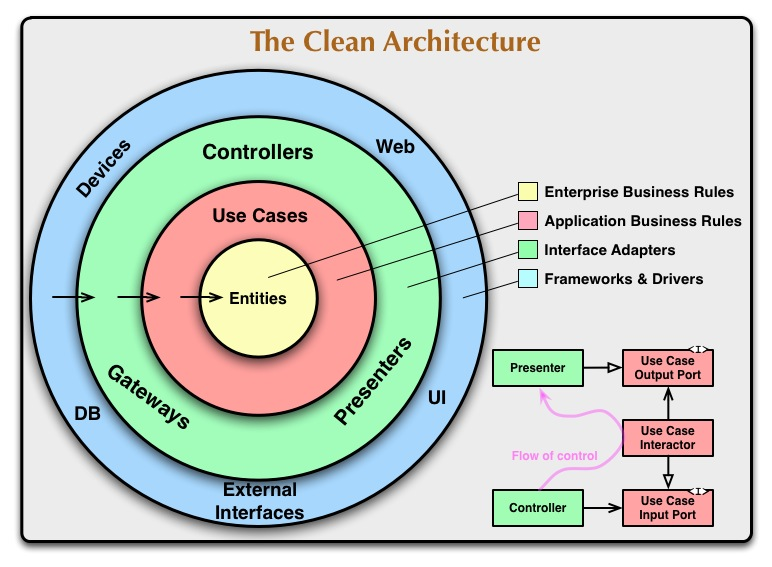
\includegraphics[scale=0.5]{CleanArchitecture}
    \caption{A arquitetura limpa}\cite{clean_arch_page}
    \label{fig:carch}
  \end{figure}
  \paragrafo{A seguir, será detalhado do que cada nível se trata nesse modelo, e, a fim 
  de elucidar cada camada, usaremos como exemplo um sistema de gerenciamento de usuários.}

  \paragrafo{Regras de Negócio de Empresa (\emph{Enterprise Business Rules}), ou as 
  Entidades, são objetos com suas próprias funções ou estruturas de dados que possam ser 
  utilizadas por várias aplicações diferentes numa mesma empresa. No contexto desse 
  trabalho e na maioria das aplicações web, as entidades serão as tabelas do banco de 
  dados, devido a sua grande tendência de reutilização em diferentes partes de um mesmo 
  sistema. No exemplo proposto, a entidade seria uma tabela de usuários com os atributos 
  do mesmo, como o nome, endereço, login e senha.}
  \paragrafo{Regras de Negócio da Aplicação (\emph{Application Business Rules}), ou os 
  Casos de Uso, são todos os fluxos especificos de uma aplicação. Essas regras de negócio 
  utilizam-se manipulam as Entidades a fim de processar o que lhes for pedido. No exemplo 
  proposto, os casos de uso seriam os algoritmos de cadastro, autenticação, consulta, 
  atualização, remoção e outras tarefas referentes à tabela previamente apresentada.}
  \paragrafo{Os Adaptadores de Interface (\emph{Interface Adapters}) tem como propósito 
  converter os dados entre os níveis vizinhos de uma forma que seja conveniente para 
  todos os envolvidos. Um exemplo de adaptador no sistema pode ser uma classe responsável 
  por tratar as requisições recebidas pelos frameworks a fim de executar os casos de uso 
  para gerenciar os usuários.}
  \paragrafo{Por fim, os Frameworks e Drivers são geralmente, no contexto de 
  desenvolvimento web, as ferramentas usadas para acesso a banco de dados e web. Por 
  serem ferramentas já prontas, geralmente só é desenvolvido nessa camada a comunicação 
  com os níveis mais internos.}
  \paragrafo{Em resumo, um sistema que separa suas preocupações e que segue a Regra da 
  Dependência tendem ter uma arquitetura limpa, com módulos de lógica de negócios 
  testáveis, independentes de frameworks, UI, banco de dados ou qualquer agência externa.}
  \end{subsecao}
  \end{secao}

  \begin{secao}{SOLID} \label{sec:solid}
    \paragrafo{Os princípios SOLID, em resumo, se tratam de regras de organização de 
    funções e estruturas de dados em agrupamentos. O principal objetivo de sua aplicação 
    está em criar software que seja de fácil entendimento, manutenção e reaproveitamento.}
    \paragrafo{Também proposto por Robert C. Martin, SOLID é um acrônimo para siglas que 
    representam princípios a serem seguidos no desenvolvimento de um bom software orientado 
    a objetos. Para exemplificar cada um desses princípios, consideremos um sistema de 
    pagamentos.}
    \begin{subsecao}{\emph{Single Responsiblity Principle}} \label{subsec:SRP}
      \paragrafo{De acordo com o \acs{SRP}, ou o Princípio da Responsabilidade Única, uma 
      classe deveria ter uma, e somente uma razão para ser alterada \cite{ood_principles}. 
      Esse princípio é relevante, pois ao dividir as responsabilidades corretamente em cada 
      módulo, evita-se consequências não planejadas durante o processo de manutenção do 
      software.} 
      \paragrafo{Exemplificando essa situação, ao desenvolver uma classe que é responsável 
      tanto por gerenciar usuários quando efetuar pagamentos, estamos quebrando esse 
      príncipio. Imagine que é realizada uma validação do usuário destinatário antes de se 
      executar um pagamento. Se houver alguma mudança nessa rotina de validação, é possível 
      que isso afete a rotina de pagamentos de formas imprevistas. A forma que seguiria o 
      \acs{SRP} seria desenvolver uma classe que fosse responsável pela gerência dos 
      usuários e outra que fosse responsável pelos pagamentos.}
    \end{subsecao}
    \begin{subsecao}{\emph{Open-Closed Principle}} \label{subsec:OCP}
      \paragrafo{O Princípio Aberto-Fechado consiste em garantir que o comportamento de uma 
      classe deveria estar aberto para a extensão, mas fechado para modificações \cite{ood_principles}.
       A importância desse princípio se deve ao fato de que ao modificar uma classe, essa 
       modificação provavelmente vai influenciar algum ponto não previsto do sistema que 
       utilize esse mesmo componente.}
      \paragrafo{No sistema exemplificado, ao acrescentar suporte à pessoas jurídicas ao 
      algoritmo de validação de usuários, se simplesmente acrescentarmos ao código 
      existente uma condição (ou um \emph{if}) para verificar o tipo da pessoa (Física ou 
      Jurídica) a fim de escolher o método de validação, estaríamos quebrando o \acs{OCP}.
      O correto seria termos uma classe abstrata Pessoa e estender esse comportamento 
      através de duas classes filhas PessoaFisica e PessoaJuridica, cada uma com seu método 
      de validação.}
    \end{subsecao}
    \begin{subsecao}{\emph{Liskov Substitution Principle}} \label{subsec:LSP}
      \paragrafo{Segundo o Princípio da Subsituição de Liskov, as classes devem ser capazes 
      de serem substituídas por suas classes derivadas sem afetar a execução do programa (e 
      vice versa). Este princípio, aliado ao \acs{OCP}, garante uma maior facilidade de 
      manutenção do código.}
      \paragrafo{Reutilizando os exemplos anteriores, o desenvolvedor estará aplicando o 
      \acs{LSP} se o mesmo passar o método de validação de uma classe Pessoa ao tentar 
      validar a PessoaFisica ou PessoaJuridica antes de realizar um pagamento.}
    \end{subsecao}
    \begin{subsecao}{\emph{Interface Segregation Principle}} \label{subsec:ISP}
      \paragrafo{No Princípio de Segregação de Interfaces define que as interfaces devem 
      ser criadas de forma granular e específica para seus clientes. Isso quer dizer que 
      não é interessante um cliente (ou classe) depender de uma interface que possui 
      métodos que o mesmo não tenha conhecimento.}
      \paragrafo{Por exemplo, havendo uma interface IPagamento e duas classes 
      PagamentoBoleto e PagamentoTed, o \acs{ISP} estaria sendo violado se houver um método 
      getLinhaDigitavel na IPagamento, visto que pagamentos via TED não usam linhas 
      digitáveis. O ideal seria que essa interface fosse melhor subdividida (ou 
      granularizada) a fim de que as classes usassem todos os seus métodos.}
    \end{subsecao}
    \begin{subsecao}{\emph{Dependency Inversion Principle}} \label{subsec:DIP}
      \paragrafo{Por fim, o Princípio da Inversão de Dependências indica que uma classe 
      deveria depender apenas de abstrações, e não de implementações. Este princípio está 
      fortemente ligado ao modelo de Arquitetura Limpa descrito na Seção \ref
      {subsec:clean-architecture}, principalmente na camada de Adaptadores e Interfaces.}
      \paragrafo{Suponha-se que o exemplificado sistema de pagamentos consuma algum serviço 
      externo para realizar alguma consulta ou validação. A estratégia de implementação da 
      chamada à esse serviço externo, seguindo o \acs{DIP}, seria criar uma interface que 
      estabelecesse o contrato com o serviço externo e usá-la no sistema de pagamentos toda 
      vez que o mesmo fosse necessário.}
      
    \end{subsecao}
    \emph{Nota: Posteriormente pretendo colocar alguns trechos de código ilustrando melhor os casos exemplificados}
  \end{secao}

\begin{secao}{Design Patterns} \label{sec:patterns}

  \paragrafo{Como alguns princípios vistos na seção de Clean Architecture, os Design Patterns tem como principal função garantir a reusabilidade do código com baixo 
  acoplamento. De fato, a proposta principal do livro está em ser um catálogo de soluções 
  para problemas de sistemas orientados a objetos.}
  \paragrafo{No total, são 23 padrões de projetos diferentes, subdividos em 3 tipos: 
  Padrões de Criação, Padrões Comportamentais e Padrões Estruturais:}
  
  \paragrafo{Padrões de Criação}
  \begin{lista}
   \itemlista{Abstract Factory}
   \itemlista{Builder}
   \itemlista{Factory Method}
   \itemlista{Prototype}
   \itemlista{Singleton}
  \end{lista}

  \paragrafo{Padrões Estruturais}
  \begin{lista}
    \itemlista{Adapter}
    \itemlista{Bridge}
    \itemlista{Composite}
    \itemlista{Decorator}
    \itemlista{Facade}
    \itemlista{Flyweight}
    \itemlista{Proxy}
  \end{lista}
  
  \paragrafo{Padrões Comportamentais}
  \begin{lista}
    \itemlista{Chain of Responsiblity}
    \itemlista{Command}
    \itemlista{Interpreter}
    \itemlista{Iterator}
    \itemlista{Mediator}
    \itemlista{Memento}
    \itemlista{Observer}
    \itemlista{State}
    \itemlista{Strategy}
    \itemlista{Template Method}
    \itemlista{Visitor}
  \end{lista}
  
  \paragrafo{Não faz parte da proposta desse trabalho usar cada um dos padrões 
  supracitados. A proposta está em identificar as oportunidades de aplicação durante as 
  etapas de desenvolvimento e expor como a adoção dos padrões solucionou o problema de uma 
  forma melhor que a não-adoção.}
  \emph{Nota: Como o sistema, até o atual momento, não está pronto, será necessário revisitar esse capítulo posteriormente listando e explicando cada padrão usado na aplicação web.}
\end{secao}

\end{capitulo}